\documentclass[10pt,a4paper]{article}
\usepackage[utf8]{inputenc}
\usepackage[T1]{fontenc}
\usepackage{amsmath,amssymb}
\usepackage{graphicx}
\usepackage{booktabs}
\usepackage[margin=1.7cm,top=1.5cm,bottom=1.5cm]{geometry}
\usepackage{hyperref}
\usepackage{enumitem}
\usepackage{titlesec}
\setlength{\parindent}{0pt}
\setlength{\parskip}{3pt}
\setlist{nosep,leftmargin=1.2em}
\titleformat{\section}{\large\bfseries}{\thesection.}{0.5em}{}
\titlespacing*{\section}{0pt}{4pt}{3pt}
\pagestyle{empty}
\newcommand{\E}{\mathbb{E}}

\begin{document}

\begin{titlepage}
\centering
\vspace*{2.5cm}
{\large Universidad de la República --- Facultad de Ingeniería}\\[0.4cm]
{\large Instituto de Matemática y Estadística (IMERL)}\\[2.2cm]
{\Huge\bfseries Modelos Estadísticos\\[4pt] para la Regresión y la Clasificación}\\[0.8cm]
{\Large Entrega 1}\\[0.3cm]
{\large Segundo semestre 2026}\\[2.5cm]
\rule{0.6\textwidth}{0.4pt}\\[0.8cm]
{\large\textbf{Integrantes}}\\[0.5cm]
\begin{tabular}{ll}
Sebastián Guigou     & C.I.\ \underline{\hspace{3.5cm}} \\[6pt]
Francisco Scaletti   & C.I.\ \underline{\hspace{3.5cm}} \\[6pt]
Dionisio Bell        & C.I.\ \underline{\hspace{3.5cm}} \\
\end{tabular}\\[0.8cm]
\rule{0.6\textwidth}{0.4pt}\\[1.2cm]
{\large Código de los tres problemas:}\\[0.2cm]
\url{https://github.com/seboongas/ModelosEst}\\[2cm]
{\large Montevideo, octubre de 2026}
\end{titlepage}

%==========================================================================
\section{Estimador de máxima verosimilitud}
La densidad es $f(x)=\tfrac12(1+\theta x)$ en $[-1,1]$ y trabajamos con $\theta=-1/3$.

\textbf{Simulación.} Para simular usamos la transformada inversa. La FDA es $F(x)=\tfrac{x+1}{2}+\theta\tfrac{x^2-1}{4}$, y al despejar $x$ de $F(x)=u$ con $u\sim U(0,1)$ nos queda $x=\bigl(-1+\sqrt{1-\theta(2-\theta-4u)}\bigr)/\theta$. Para chequear que funciona, simulamos $2\cdot10^5$ datos: el histograma se pega a $f$ (Fig.~1, izquierda) y la media dio $-0{,}114$, muy cerca de $\E[X]=\theta/3=-0{,}111$.

\textbf{Verosimilitud.} La log-verosimilitud es $\ell(\theta)=\sum_i\log(1+\theta x_i)-n\log 2$. Es cóncava en $\theta$ (la segunda derivada es $-\sum_i x_i^2/(1+\theta x_i)^2<0$), así que hay un único máximo y la búsqueda de la sección áurea sobre $[-1,1]$ lo encuentra. Implementamos el golden search a mano y lo comparamos con \texttt{scipy.optimize.minimize\_scalar}, que dio lo mismo. Acá no hay una fórmula cerrada para $\hat\theta$, por eso hace falta optimizar numéricamente.

\begin{center}
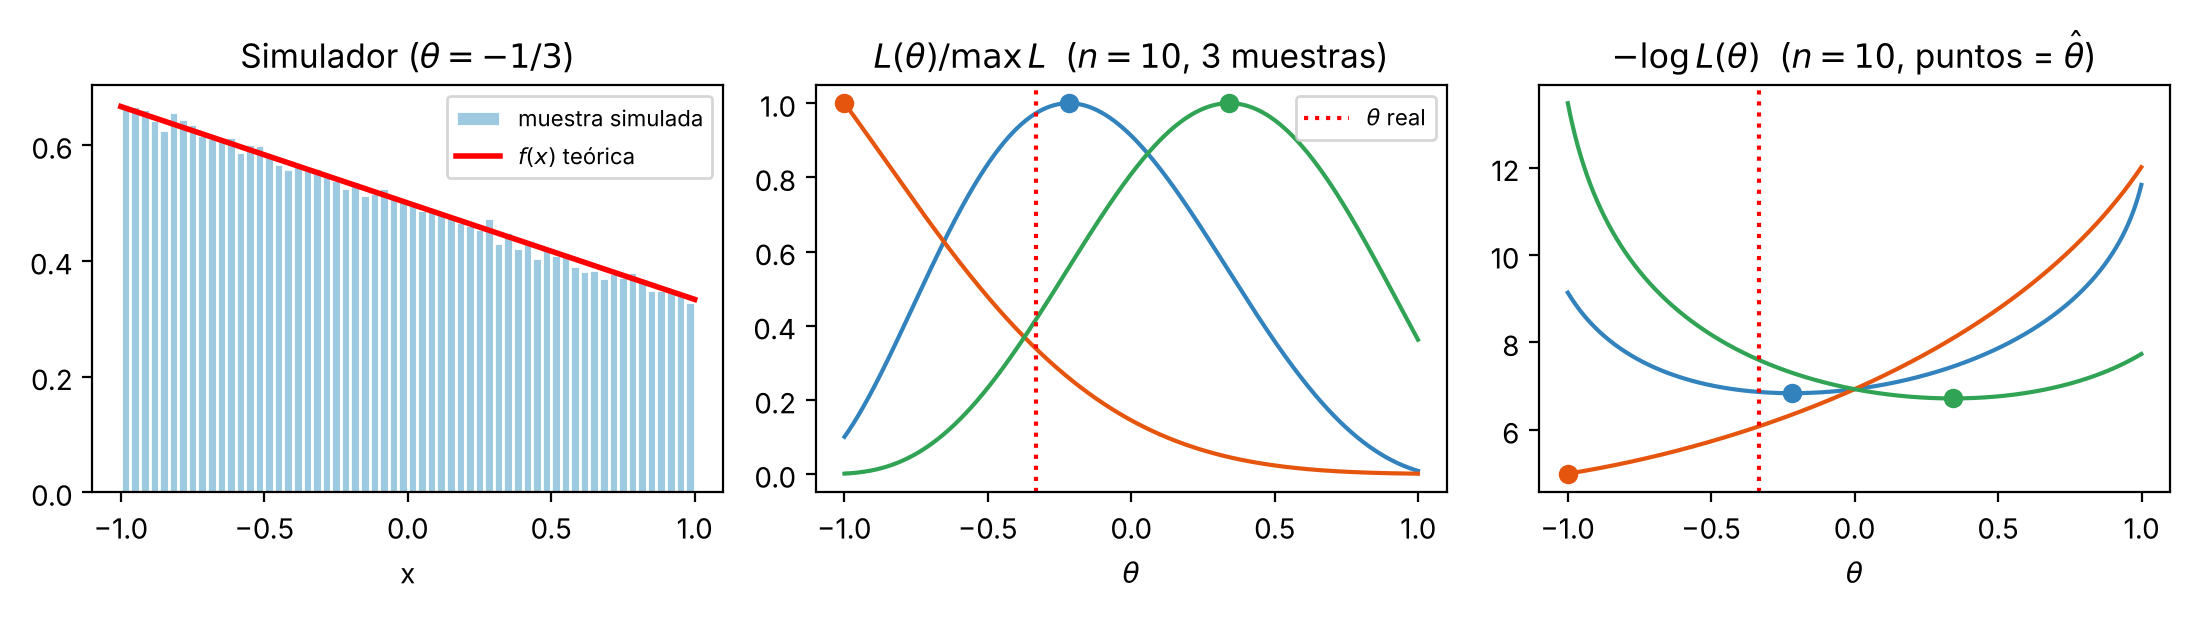
\includegraphics[width=\textwidth]{../figuras/p1_verosimilitud.png}\\
{\small Figura 1. Simulador y verosimilitud para tres muestras de tamaño 10 (los puntos marcan cada $\hat\theta$).}
\end{center}

Con $n=10$ el máximo cambia bastante de una muestra a otra: en la Fig.~1 dieron $\hat\theta=-0{,}22$, $-1$ y $0{,}34$. Cuando la verosimilitud es monótona en $[-1,1]$ el máximo queda en el borde ($\hat\theta=\pm1$), y eso pasó en cerca del 19\,\% de las muestras de tamaño 10.

\textbf{Sesgo, varianza y MSE.} Generamos $M=1000$ muestras para cada $n$ y calculamos $\hat\theta$ en cada una, con $\mathrm{MSE}=\text{sesgo}^2+\text{varianza}$. La letra sugiere unas 50 muestras, pero probamos con $M=50$ y $n=10$ y el sesgo dio $0{,}16$, que es puro ruido de la simulación (su error estándar es de $\approx0{,}07$). Por eso usamos 1000.

\begin{center}
\small
\begin{tabular}{rrrrrr}
\toprule
$n$ & media de $\hat\theta$ & sesgo & varianza & MSE & $n\cdot$var \\
\midrule
10   & $-0{,}345$ & $-0{,}012$ & $0{,}2738$ & $0{,}2739$ & $2{,}74$ \\
100  & $-0{,}333$ & $\phantom{-}0{,}001$ & $0{,}0279$ & $0{,}0279$ & $2{,}79$ \\
1000 & $-0{,}332$ & $\phantom{-}0{,}001$ & $0{,}0028$ & $0{,}0028$ & $2{,}84$ \\
\bottomrule
\end{tabular}
\end{center}

\begin{center}
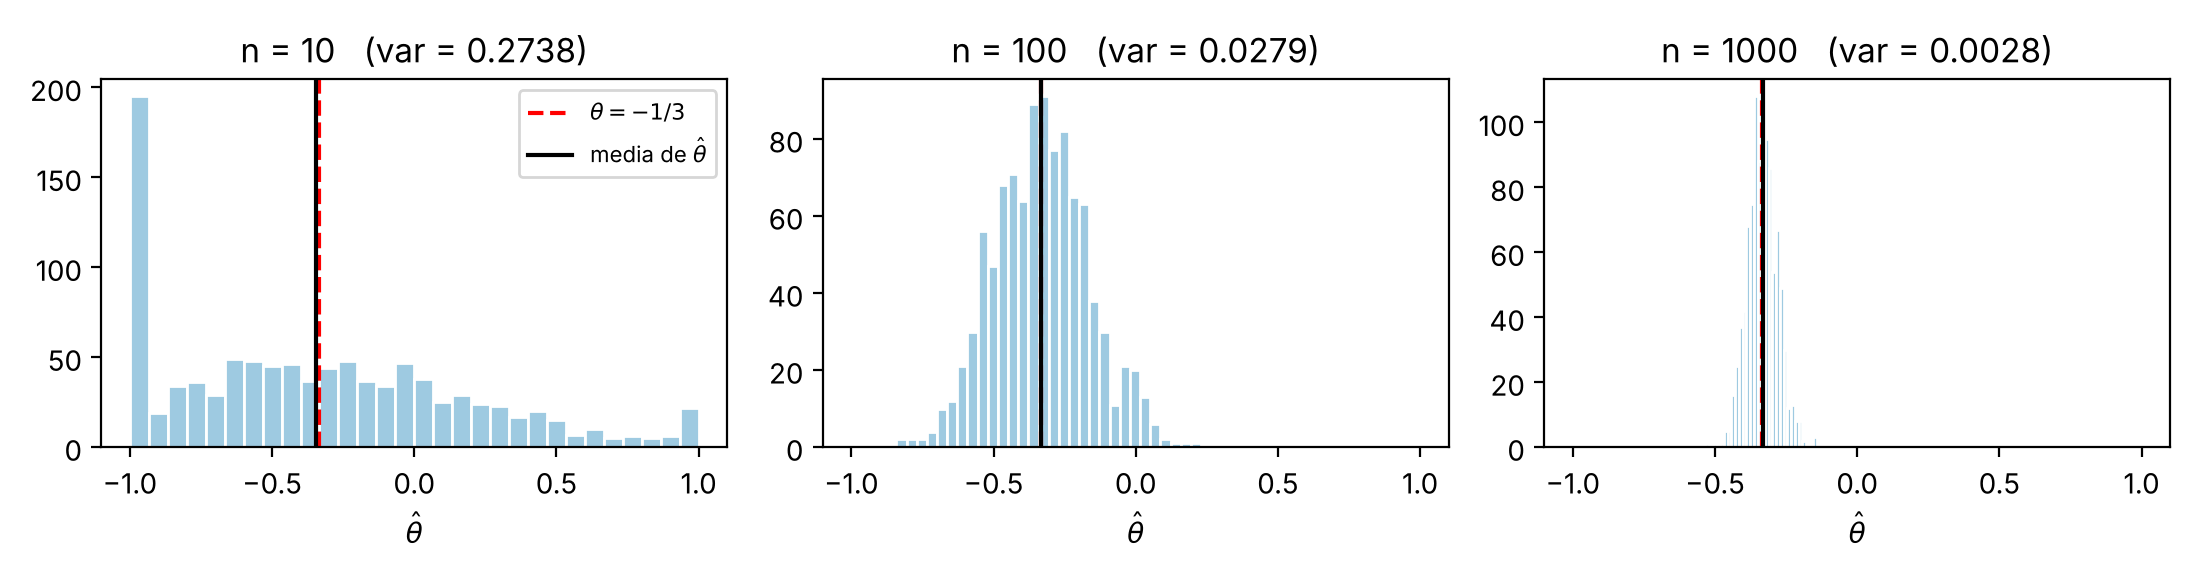
\includegraphics[width=\textwidth]{../figuras/p1_distribucion_estimador.png}\\
{\small Figura 2. Distribución de $\hat\theta$ en las 1000 muestras, para cada $n$ (la línea roja es $\theta=-1/3$).}
\end{center}

\textbf{Conclusiones.} El sesgo es chico en los tres casos: queda dentro de un error estándar de la simulación ($0{,}017$; $0{,}005$ y $0{,}002$), así que no podemos distinguirlo de cero. Esto va con que el MLE es asintóticamente insesgado. Lo que sí cambia mucho es la varianza: se divide por 10 cada vez que $n$ se multiplica por 10. De hecho $n\cdot\mathrm{var}$ queda cerca de $2{,}8$, que es $1/I(\theta)$ con $I(\theta)=\tfrac12\int_{-1}^1\tfrac{x^2}{1+\theta x}dx=0{,}3575$ (la información de Fisher). Como el sesgo es casi nulo, el MSE es básicamente la varianza. Además, con $n=10$ la distribución de $\hat\theta$ no se parece a una normal porque se amontona en $\pm1$, mientras que con $n\ge100$ ya se ve parecida a una normal centrada en $-1/3$.

\newpage
%==========================================================================
\section{Regresión en Boston Housing}
\textbf{Datos y exploración.} Usamos el dataset \texttt{Boston} del paquete ISLP (506 viviendas, 12 atributos y \texttt{medv}, sin datos faltantes). Esta versión no trae la variable \texttt{B} del dataset original. \texttt{medv} tiene la cola larga hacia la derecha y 16 viviendas valen exactamente 50, que parece ser un tope. Las variables más correlacionadas con \texttt{medv} son \texttt{lstat} ($-0{,}74$), \texttt{rm} ($0{,}70$) y \texttt{ptratio} ($-0{,}51$). La relación con \texttt{lstat} se ve claramente curva, lo cual es una buena razón para probar polinomios.

\begin{center}
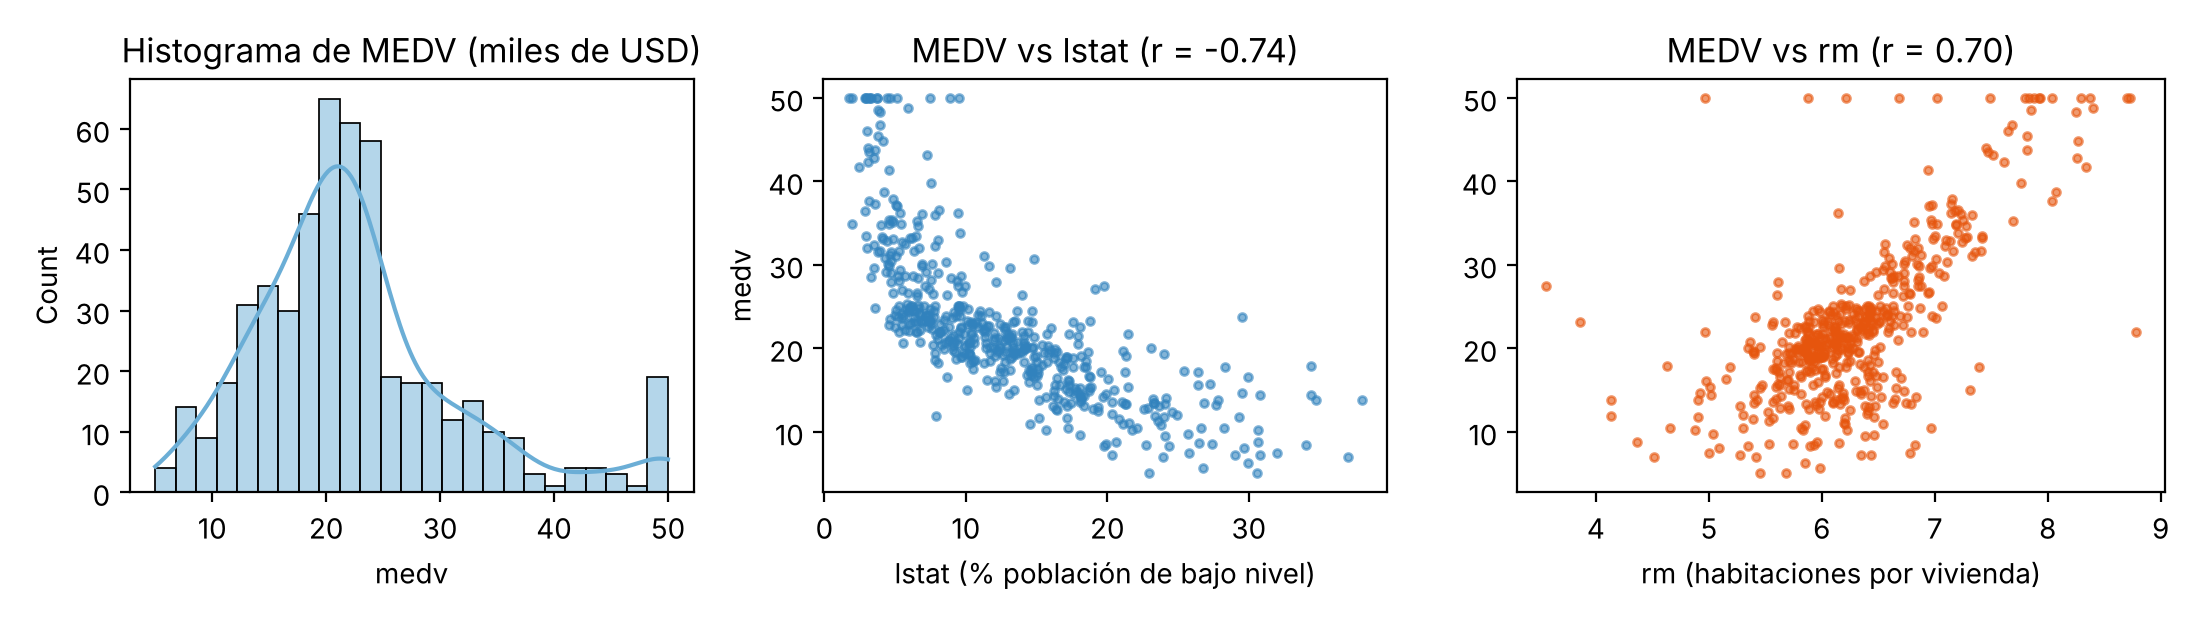
\includegraphics[width=0.92\textwidth]{../figuras/p2_eda.png}\\
{\small Figura 3. Exploración inicial: distribución de MEDV y las dos relaciones más fuertes.}
\end{center}

\textbf{Qué hicimos.} Separamos los datos al azar en 80\,\% para entrenamiento (404) y 20\,\% para validación (102), con semilla 42. Todos los modelos siguen el mismo esquema: características polinomiales, estandarización y regresión (MCO o Ridge). El $\lambda$ de Ridge lo elegimos con validación cruzada de 5 folds usando solo el conjunto de entrenamiento, para no usar la validación en la elección. Tengamos en cuenta que con grado 3 hay 454 atributos y solo 404 observaciones.

\begin{center}
\small
\begin{tabular}{c r rr c rrr}
\toprule
 & & \multicolumn{2}{c}{MCO (sin regularizar)} & & \multicolumn{3}{c}{Ridge ($\lambda^*$ por CV)}\\
\cmidrule{3-4}\cmidrule{6-8}
Grado & \#atrib. & MSE entr. & MSE valid. & $\lambda^*$ & MSE CV & MSE entr. & MSE valid.\\
\midrule
1 & 12  & 22,60 & 22,78   & 3,98 & 25,28 & 22,62 & 22,91 \\
2 & 90  & 5,72  & 15,16   & 0,40 & \textbf{16,07} & 6,80 & 11,94 \\
3 & 454 & 0,46  & 1175,60 & 1,00 & 18,06 & 4,22 & 10,73 \\
\bottomrule
\end{tabular}
\end{center}

\begin{center}
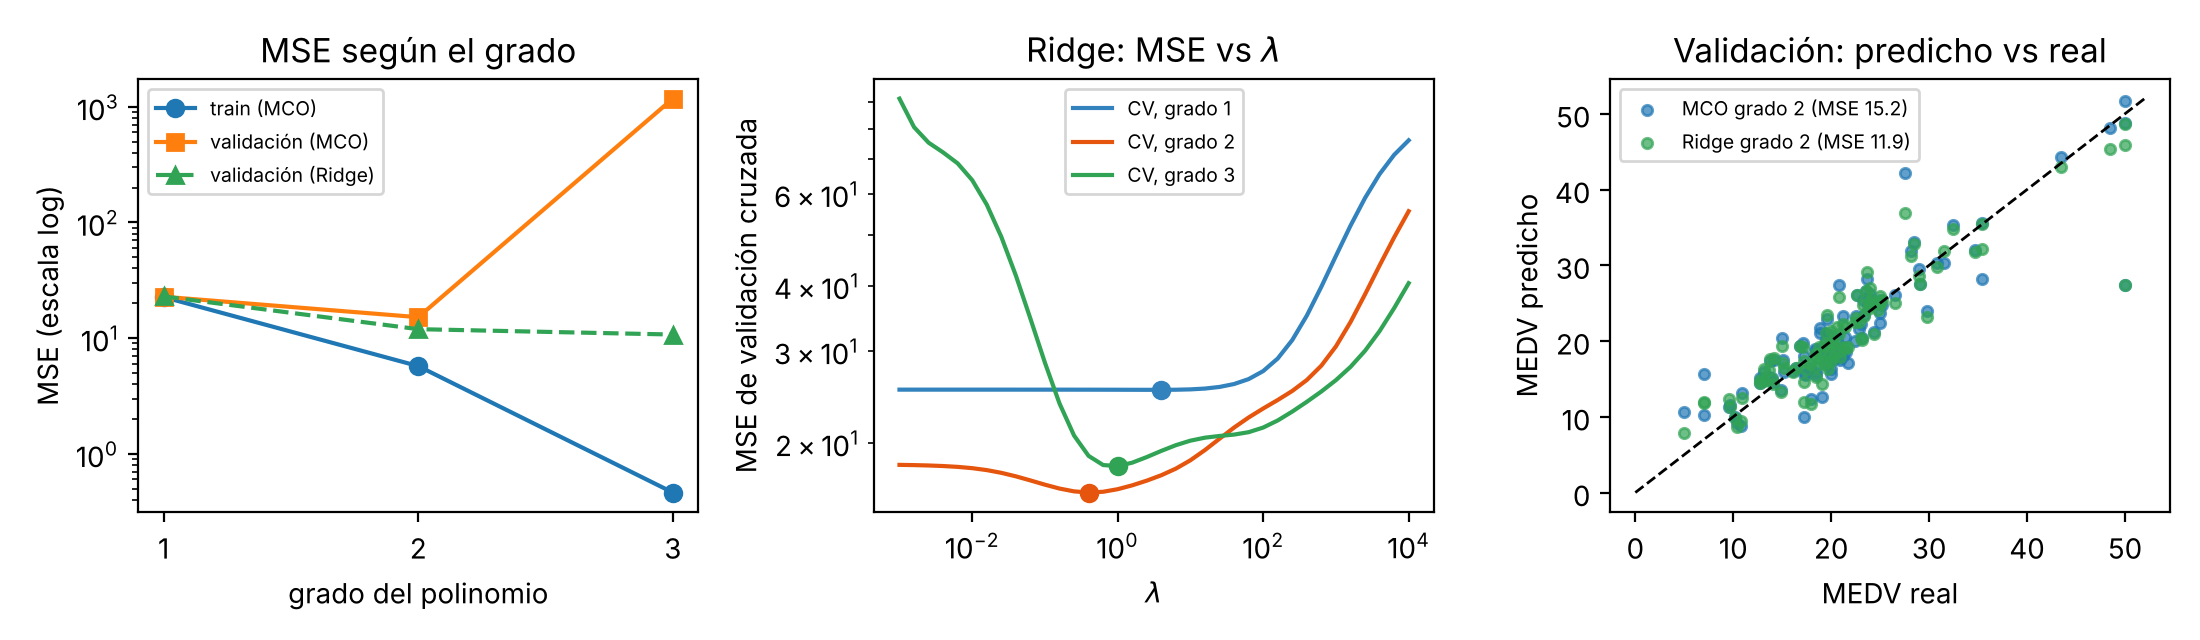
\includegraphics[width=\textwidth]{../figuras/p2_resultados.png}\\
{\small Figura 4. Izquierda: MSE según el grado. Centro: MSE de validación cruzada en función de $\lambda$ (el punto es el mínimo). Derecha: predicho vs.\ real en validación, para MCO de grado 2 y Ridge de grado 2.}
\end{center}

\textbf{Conclusiones.} El modelo lineal tiene un MSE parecido en entrenamiento y validación (22,6 y 22,8), o sea que no sobreajusta, pero tampoco captura la curvatura que vimos en los datos. Con grado 2 el MSE de validación baja a 15,2, aunque ya aparece una diferencia grande con el de entrenamiento (5,7). Con grado 3 y MCO el modelo tiene más atributos que datos, interpola el entrenamiento (MSE 0,46) y en validación explota a 1176, que es sobreajuste total.

Ridge arregla justamente ese problema. Con grado 2 el MSE de validación baja de 15,2 a 11,9, y con grado 3 pasa de 1176 a 10,7. En grado 1 casi no cambia nada, lo cual tiene sentido porque con solo 12 atributos no hay mucho que penalizar.

Para nosotros el mejor modelo es Ridge con polinomio de grado 2 y $\lambda\approx0{,}4$, porque tiene el menor MSE de validación cruzada (16,1 contra 18,1 del grado 3). En esta partición el grado 3 con Ridge dio un MSE de validación un poco menor (10,7 contra 11,9), así que para ver si era una diferencia real repetimos todo con 30 particiones al azar. Ahí las medianas fueron 11,7 (grado 2) y 12,3 (grado 3), con desvíos de 3,8 y 5,6, o sea que la diferencia se pierde en el ruido y nos quedamos con el más simple. Como referencia, la mediana del MCO de grado 3 en esas particiones fue 1681.

Una limitación: como el valor máximo de \texttt{medv} está cortado en 50, el modelo subestima esas viviendas (se ven los puntos de abajo a la derecha en la Fig.~4). Además, el MSE de una sola partición es bastante ruidoso.

\newpage
%==========================================================================
\section{Alturas}
\textbf{Datos y decisiones.} Hay 45 respuestas. Sacamos 2: el id 36 no tiene la altura del estudiante y el id 4 no tiene el sexo. Quedaron 43 (36 varones y 7 mujeres). La altura depende mucho del sexo (en promedio 179,2 cm los varones y 162,9 cm las mujeres), así que lo incluimos como variable indicadora. No agregamos pendientes distintas por sexo (interacciones) porque hay apenas 7 mujeres, y además ese modelo salió peor en el error de validación cruzada leave-one-out (29,1 contra 21,6) y en el AIC. Comparamos varios modelos con el $R^2$ ajustado, el AIC y ese error LOO:

\begin{center}
\small
\begin{tabular}{lrrrr}
\toprule
Modelo para la altura del estudiante & $R^2$ ajust. & AIC & $\hat\sigma$ (cm) & ECM LOO \\
\midrule
padre                      & 0,02 & 301,1 & 7,84 & 65,8 \\
padre + madre              & 0,02 & 302,1 & 7,85 & 67,2 \\
sexo                       & 0,58 & 264,3 & 5,11 & 28,3 \\
padre + sexo               & 0,66 & 255,8 & 4,58 & 23,7 \\
\textbf{padre + madre + sexo} & \textbf{0,71} & \textbf{251,1} & \textbf{4,29} & \textbf{21,6} \\
padre + madre + sexo + interacciones & 0,69 & 254,8 & 4,39 & 29,1 \\
\bottomrule
\end{tabular}
\end{center}

Una cosa que nos llamó la atención es que sin el sexo las alturas de los padres no explican nada ($R^2$ ajustado de 0,02). Recién aportan cuando se controla por sexo.

\begin{center}
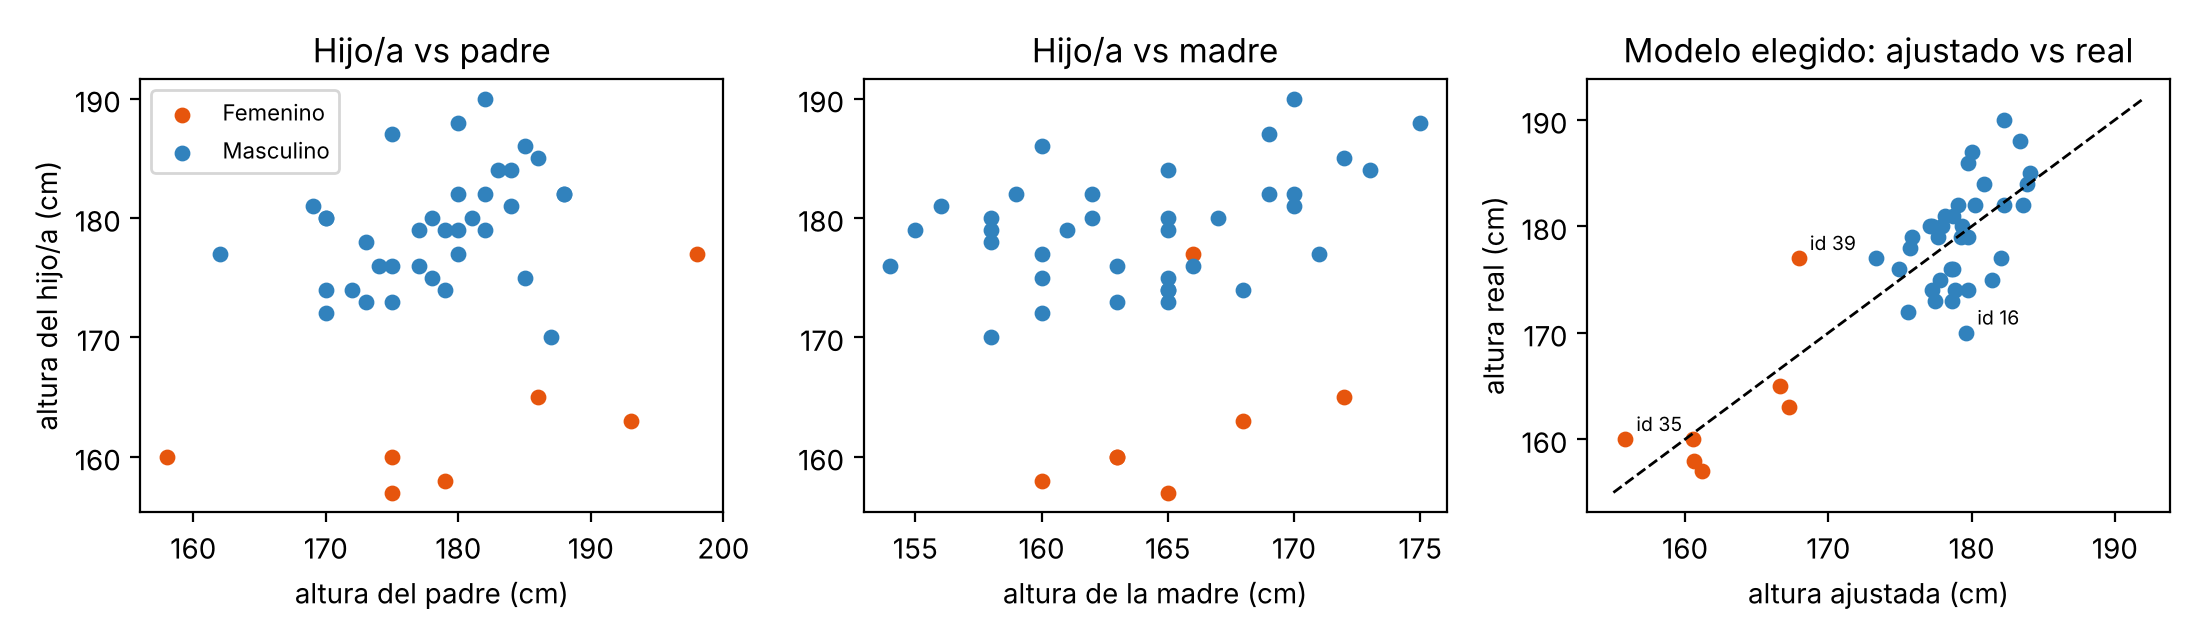
\includegraphics[width=\textwidth]{../figuras/p3_alturas.png}\\
{\small Figura 5. Altura del estudiante contra la del padre y la de la madre (por sexo), y ajustado vs.\ real del modelo elegido.}
\end{center}

\textbf{Modelo elegido.} Ajustamos por mínimos cuadrados con las 43 observaciones ($\hat\sigma=4{,}3$ cm, $R^2$ ajustado $0{,}71$; los residuos no muestran señales de alejarse de la normalidad):
\[
\widehat{\text{altura}} \;=\; 74{,}4 \;+\; 0{,}278\,\text{padre} \;+\; 0{,}337\,\text{madre} \;-\; 17{,}4\,\text{mujer}
\]
con las alturas en cm y $\text{mujer}=1$ si el estudiante es de sexo femenino y 0 si es masculino. Los intervalos de confianza del 95\,\% van entre corchetes.

\textbf{Qué significa cada coeficiente.}
\begin{itemize}
\item \textbf{Padre, $0{,}28$ [0,10; 0,46]:} si la madre y el sexo se mantienen fijos, un cm más de altura del padre se asocia con $0{,}28$ cm más de altura del estudiante.
\item \textbf{Madre, $0{,}34$ [0,07; 0,60]:} lo mismo pero con la madre, dejando fijos el padre y el sexo.
\item \textbf{Mujer, $-17{,}4$ [$-21{,}1$; $-13{,}8$]:} con padre y madre de la misma altura, las mujeres miden en promedio $17{,}4$ cm menos que los varones.
\item \textbf{Constante, $74{,}4$:} sería la altura esperada de un varón con padre y madre de 0 cm, así que no tiene interpretación real. Si centramos las alturas de los padres en sus promedios (178,5 y 164,2 cm), la constante pasa a ser $179{,}4$ cm: la altura esperada de un varón con padres de altura promedio.
\end{itemize}

\textbf{Conclusiones.} Los coeficientes de padre y madre suman $0{,}62$, menor que 1: un estudiante con padres muy altos tiende a ser alto, pero menos que ellos, lo que se parece a la regresión a la media. Son asociaciones y no hay que leerlas como efectos causales.

Con solo 43 datos el modelo es frágil. El id 39 (mujer de 177 cm con padre de 198 cm) es el punto más influyente, con distancia de Cook 0,57 (el umbral orientativo $4/n$ es 0,09). Si lo sacamos, el coeficiente del padre baja de 0,28 a 0,19 y el $R^2$ ajustado sube a 0,75. Decidimos dejarlo porque los datos son plausibles (el padre es muy alto) y no hay motivo para pensar que es un error de carga. El id 16 (varón de 170 cm con padre de 187 cm) es el otro residuo grande. También probamos agregar el id 4 como varón, y ahí el coeficiente de la madre baja de 0,34 a 0,17, o sea que es el menos estable de todos. Por último, los datos son de estudiantes del curso y no una muestra aleatoria, así que no conviene extrapolar el modelo a otra población.

\end{document}
